% Preamble
\documentclass[a4paper, 12pt]{article}
\usepackage[margin=1in]{geometry} % Set margin
\usepackage{pdfpages} % Insert pdf pages
\usepackage{amssymb,amsmath,amsthm, amsfonts} % Math libraries


% Custom commands
\newcommand{\sub}[1]{\subsection{\underline{#1}}}
\newcommand{\subsub}[1]{\subsubsection{\underline{#1}}}
\newcommand{\?}{\stackrel{?}{=}}
\newcommand{\R}{\ensuremath{\mathbb{R}}}
\newcommand{\F}{\ensuremath{\mathbb{F}}}
\newcommand{\eqbcuz}[1]{\text{~$\stackrel{(#1)}{=}$~}}
\renewcommand{\qed}{$$\blacksquare$$}
\renewcommand{\b}[1]{\textbf{#1}}
\renewcommand{\because}[1]{~\b{(#1)}\\}
\renewcommand{\d}{\ensuremath{\Downarrow\\~}}

% Begin Document %
\begin{document}

% Title Page
\begin{titlepage}
    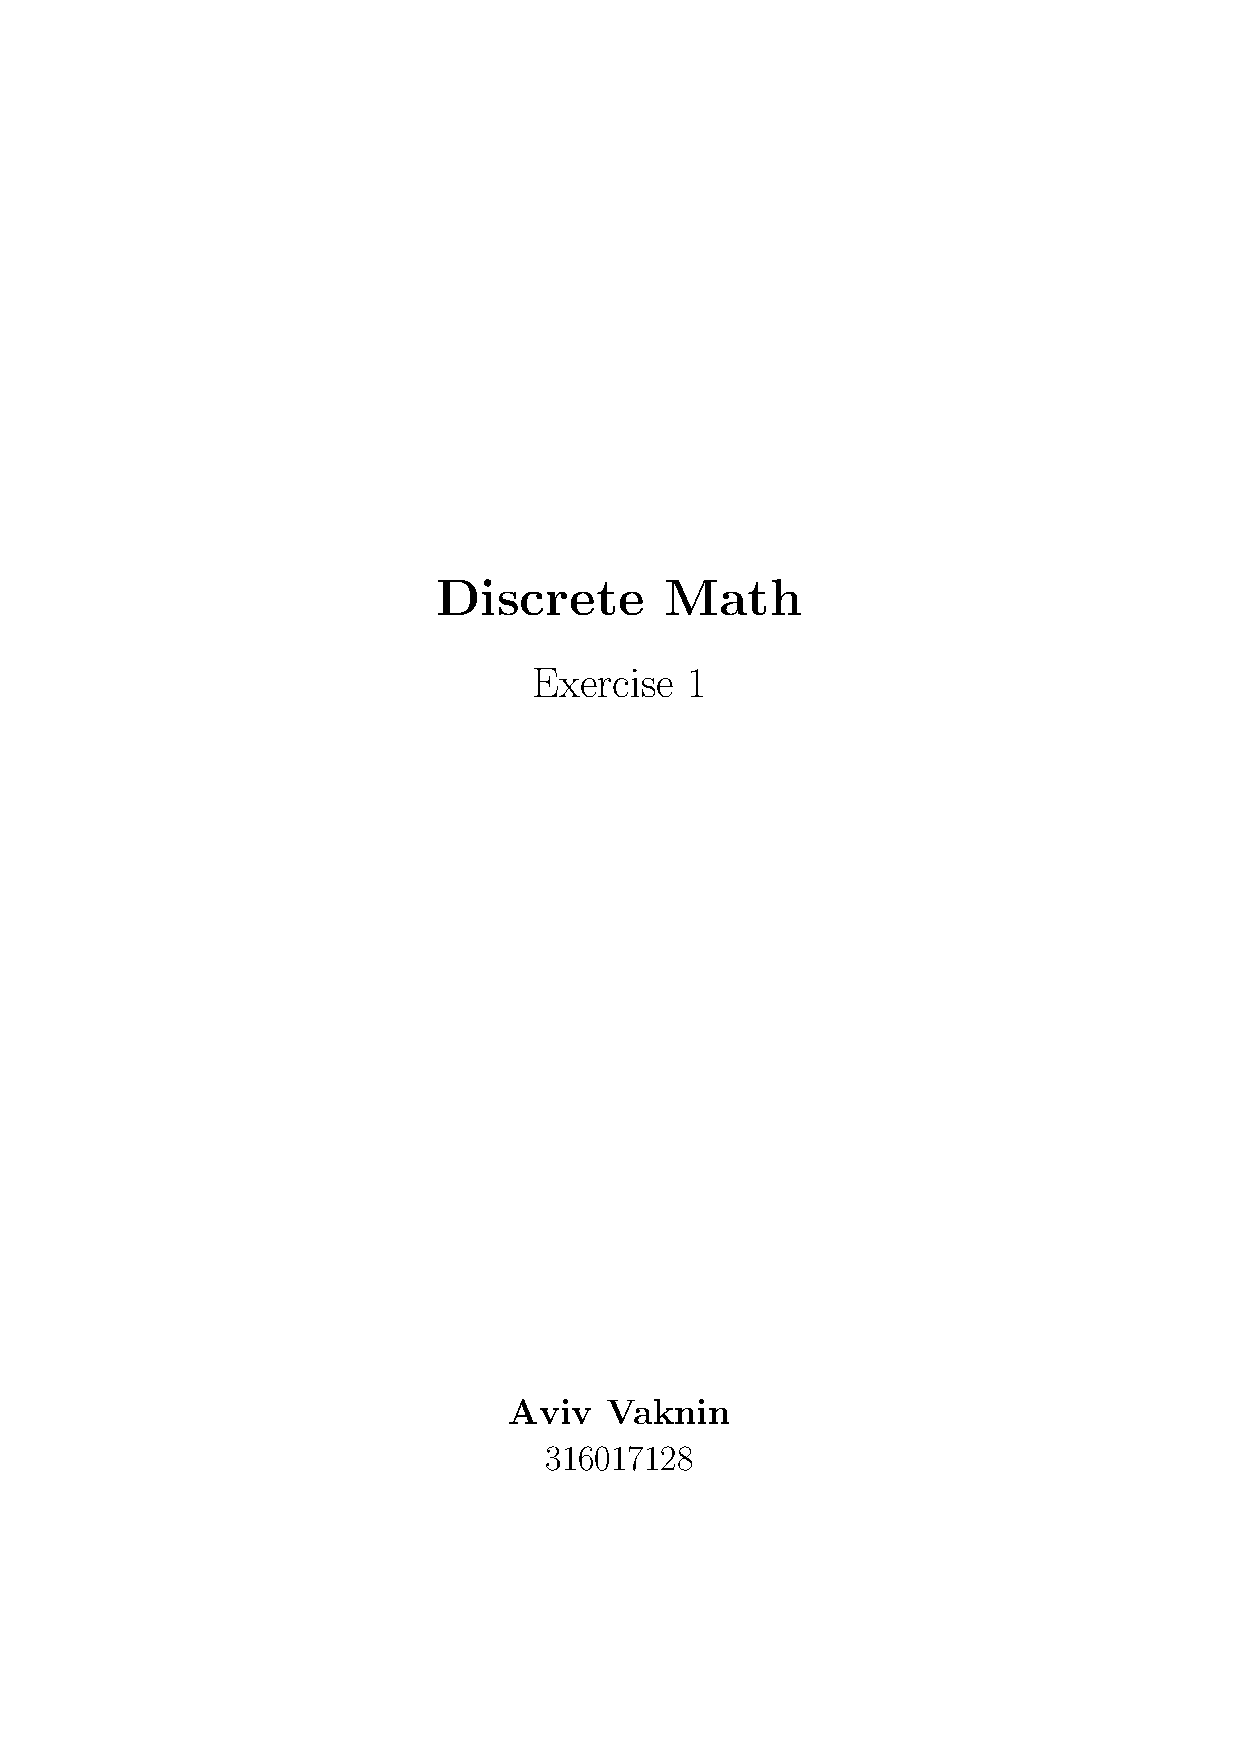
\includepdf{title.pdf}
\end{titlepage}

%1
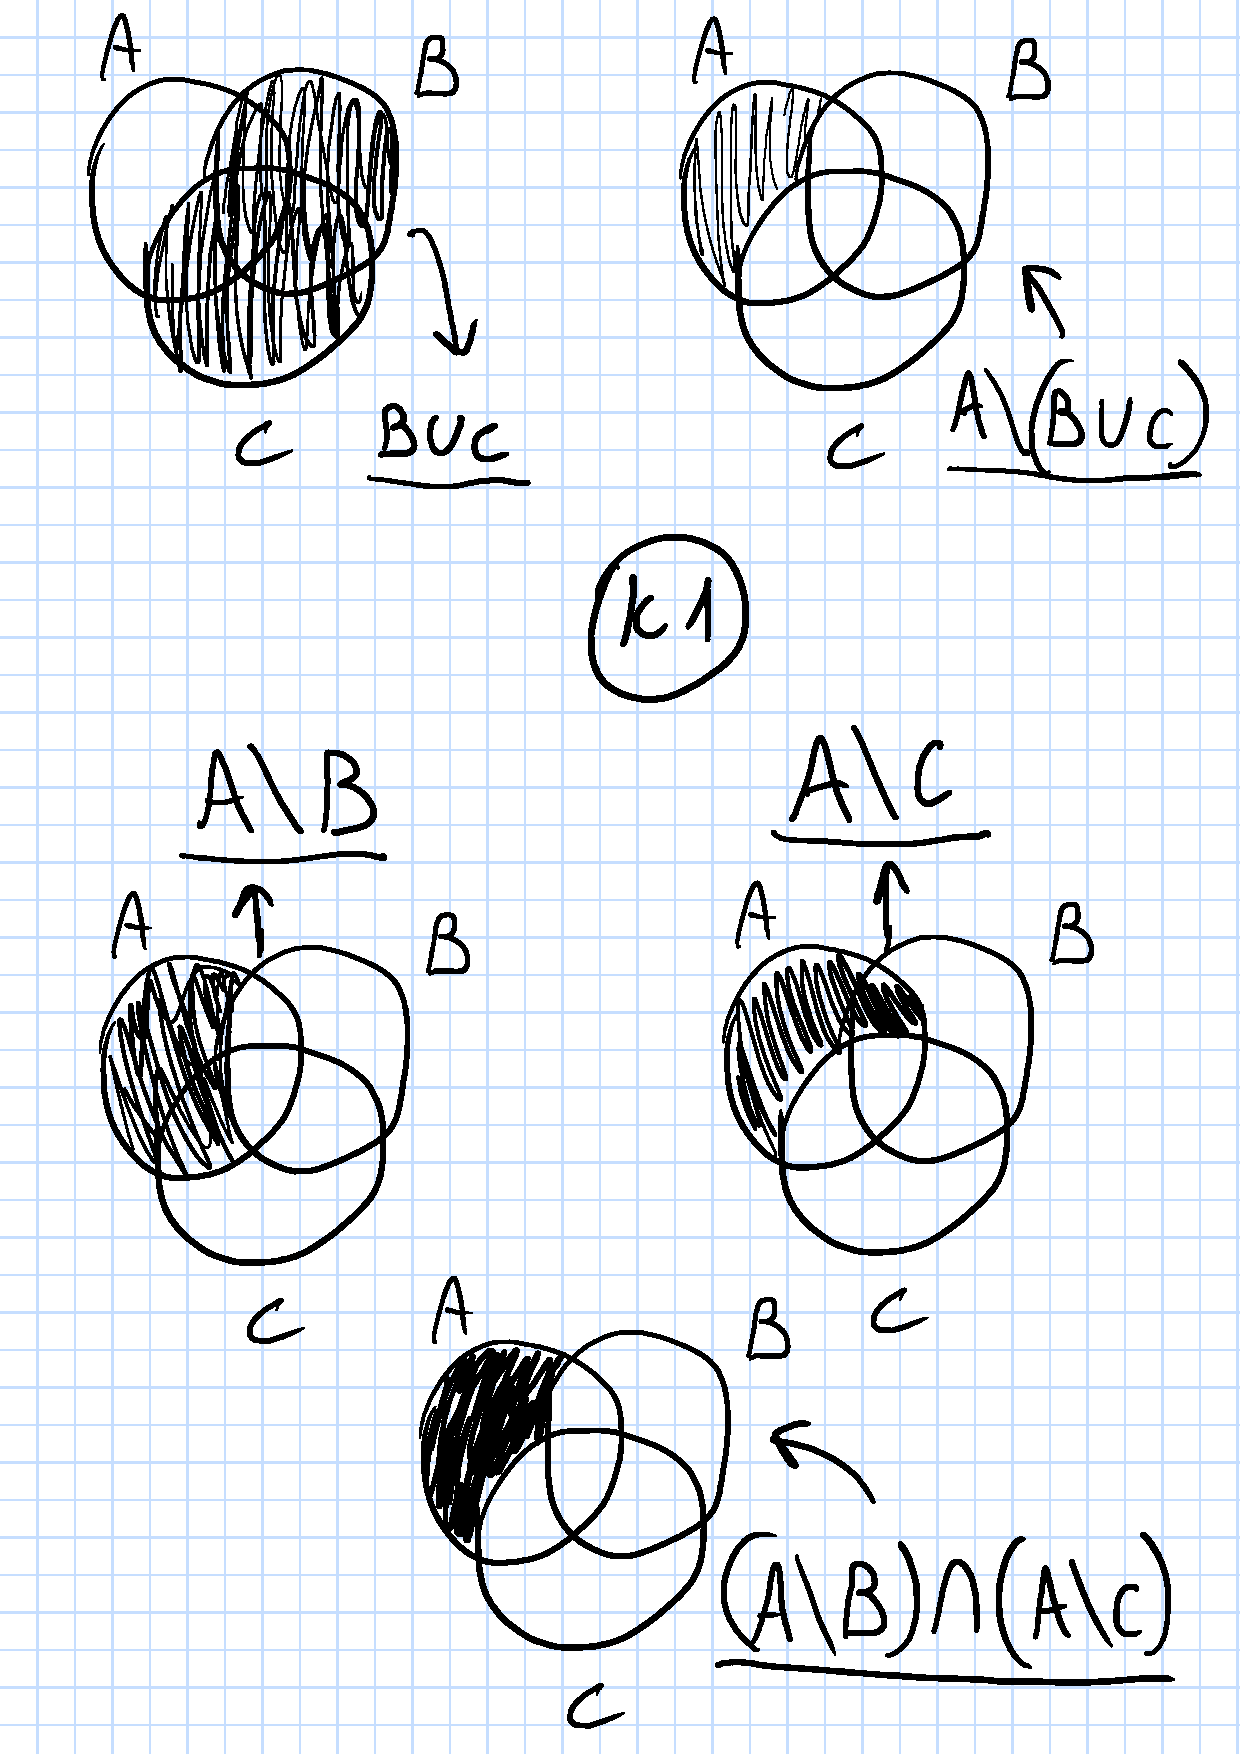
\includepdf[pages=-]{d.pdf}

% 2
\setcounter{section}{1}
\section{}
This doesn't apply for every group of sets $A,B,C$.
To prove that, let's take:
$$ A = \big{\{}1,2,3,4 \big{\}} $$
$$ B = \big{\{}3,4,5,6 \big{\}} $$
$$ C = \big{\{}2,4,6,7 \big{\}} $$
Let's create a new group, $D$, such that:
$$ D = A  \backslash (B\cap{C}) =  A  \backslash \big{\{}4,5,6 \big{\}} = \big{\{}1,2,3 \big{\}}$$
And create a new group, $E$, such that:
$$ E = (A\cup{B}) \backslash{C} =  \big{\{}1,2,3,4,5,6 \big{\}} \backslash{C} = \big{\{}1,3,5 \big{\}}$$
We can see that $ D \not\subset E $, and that $ E \not\subset D $.
\qed

%3
\section{Build a truth table for $P\rightarrow(\neg{Q}\land{R})$:}
\begin{center}
    ~\\
    \begin{tabular}{|c|c|c|c|c|c|} 
    \hline
    $P$ & $Q$ & $\neg{Q}$ & $R$ & $\neg{Q}\land{R}$ & $ P\rightarrow(\neg{Q}\land{R})$ \\ [0.5ex] 
    \hline
    T & T & F & T & F & F \\
    \hline
    T & T & F & F & F & F \\
    \hline
    T & F & T & T & T & T \\
    \hline
    T & F & T & F & F & F \\
    \hline
    F & T & F & T & F & T \\
    \hline
    F & T & F & F & F & T \\
    \hline
    F & F & T & T & T & T \\
    \hline
    F & F & T & F & F & T \\
    \hline
   \end{tabular}
\end{center}
\pagebreak

%4א
\section{Check if $A \iff B$}
P.S I will never build \LaTeX~tables again, that's just horrible.
\sub{}
We can notice that $A$ and $B$ are not equal.
\begin{center}
    ~\\
    \begin{tabular}{|c|c|c|c|c|c|c|c|} 
    \hline
    $P$ & $Q$ & $R$ & $P\Leftrightarrow{Q}$ & $(P\Leftrightarrow{Q})\land{R}~\b{[A]}$ & $P\land{R}$ & $Q\land{R}$ & $P\land{R} \Leftrightarrow Q\land{R}~\b{[B]}$ \\ [0.5ex] 
    \hline
    T & T & T & T & T & T & T & T\\
    \hline
    T & T & F & T & F & F & F & T\\
    \hline
    T & F & T & F & F & T & F & F\\
    \hline
    T & F & F & F & F & F & F & T\\
    \hline
    F & T & T & F & F & F & T & F\\
    \hline
    F & T & F & F & F & F & F & T\\
    \hline
    F & F & T & T & T & F & F & T\\
    \hline
    F & F & F & T & F & F & F & T\\
    \hline
   \end{tabular}
\end{center}

\sub{}
We can notice that $A$ and $B$ are equal.
\begin{center}
    ~\\
    \begin{tabular}{|c|c|c|c|c|c|c|c|} 
    \hline
    $P$ & $Q$ & $R$ & $P\Leftrightarrow{Q}$ & $(P\Leftrightarrow{Q})\lor{R}~\b{[A]}$ & $P\lor{R}$ & $Q\lor{R}$ & $P\lor{R} \Leftrightarrow Q\lor{R}~\b{[B]}$ \\ [0.5ex] 
    \hline
    T & T & T & T & T & T & T & T\\
    \hline
    T & T & F & T & T & T & T & T\\
    \hline
    T & F & T & F & T & T & T & T\\
    \hline
    T & F & F & F & F & T & F & F\\
    \hline
    F & T & T & F & T & T & T & T\\
    \hline
    F & T & F & F & F & F & T & F\\
    \hline
    F & F & T & T & T & T & T & T\\
    \hline
    F & F & F & T & T & F & F & T\\
    \hline
   \end{tabular}
\end{center}

\section{Is the statement correct?}
\sub{No, contradictory example: $x=5$}
\sub{Yes, for example: $x=9$}
\sub{Yes, for example: $x=6$}
\sub{No, contradictory example: $x=4$}
\pagebreak

\section{$A=\big{\{} 1,2,3 \big{\}} ~B=\big{\{}3,4,5,6 \big{\}}$}
\sub{$\forall{x}\in{A}~\exists{y}\in{B}~ x+y<7$}
This statement is true.

\sub{$\exists{x}\in{A}~\forall{y}\in{B}~ x+y<7$}
This statement is false.
For example, $1+6\not<7$.

% End Document %
\end{document}